
\section{Introduction}
\label{sec:introduction}

In this paper, we investigate \emph{tiebreaking strategies} for cost-optimal \astar.
% In optimal search, tiebreaking strategies does not affect the optimality
% of the search algorithms because they only affect the node expansion
% order among the nodes with the same $f$-cost.
% \subsection{Tiebreaking for \astar}
% This paper is organized as follows.
% After defining some notations in \refsec{sec:preliminaries}, 
% We first investigate the conventional
% tiebreaking strategies for the optimal search using \astar.
\astar is the standard search algorithm for finding an optimal cost path from an initial state $s$ to some goal
state $g \in G$ in a search space represented as a graph \cite{hart1968formal}.
It expands the nodes in the best-first order of $f(n)$ until up to $f^*$,
where $f(n)$ is a lower bound of the cost of the shortest path that contains a node $n$ and $f^*$ is the optimal cost.
% 
In many combinatorial search problems, the size of the last layer $f(n)=f^*$ of the search, called a \emph{final plateau},
accounts for a significant fraction of the effective search space of \astar.  \refig{fig:plateau-noh}
(\refpage{fig:plateau-noh}) compares the number of states in this final plateau with $f(n) = f^*$ (y-axis)
vs. $f(n) \leq f^*$ (x-axis) for 1104 problem instances from the International Planning Competition (IPC1998-2011).
For many instances, a large fraction of the nodes in the effective search space have $f(n)=f^*$: The points
are located very close to the diagonal line ($x=y$), indicating that almost all states with $f(n) \leq f^*$ have cost
$f^*$.

\refig{fig:plateau-0} depicts the conceptual view of this phenomenon.
% 
One natural  % avoiding ``naive'' here because we don't want to Frontier Search people to misunderstand and belive that we're calling them naive.
view of the search space (left) would consider the space searched by \astar as
a large number of closed nodes with $f<f^*$, surrounded by a
a thin layer of final plateau $f(n)=f^*$.  This intuitive view
may accurately describe some real, practical search spaces such as 2D pathfinding on an explicit
graph. This view has also served as the algorithms such as Frontier Search
\cite{korf1999divide,korf2000divide}, which tries to reduce the memory requirement by discarding the information associated with states with 
$f<f^*$, which can be effective when the number of states with $f<f^*$ accounts for a large fraction of the search effort.
% 
However, for many other classes of combinatorial search problems, e.g., the IPC Planning Competition Benchmarks, 
the figure on the right is a more accurate depiction -- here, the  search space has a large plateau for $f=f^*$.
In fact, Iterative Deepening approaches \cite{korf1985depth} assume this type of search space
where this final frontier is quite huge and the cost of re-evaluating $f<f^*$ is limited.
Classical planning problems in IPC benchmarks are clearly the instances of such combinatorial search problems.
\todo*{The fact that the last layer of search dominates the search was the motivation for Frontier Search and its numerous variants, so the SoCS community has been well aware of this --- SoCS community considers the opposite. Frontier search would not gain advantage in the planning domains because the number of nodes being forgotten is low compared to the size of the plateau.}

\begin{figure}[htbp]
  \centering
  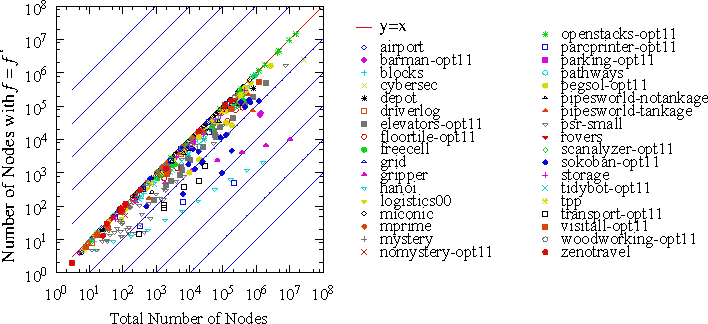
\includegraphics[width=\linewidth]{tables/aaai16-frontier/aaai16prelim3/lmcut_frontier_noh-front.pdf}
 \caption{
 The number of nodes with $f=f^*$ (y-axis) compared to the
 total number of nodes in the search space (x-axis) with $f\leq f^*$ on 1104 IPC benchmark problems.
 This experiment uses a modified Fast Downward with \lmcut which 
 continues the search within the current $f$ after any cost-optimal solution is found.
 This effectively generates all nodes with cost $f^*$.
  }
 \label{fig:plateau-noh}
\end{figure}

\begin{figure}[htbp]
  \centering
  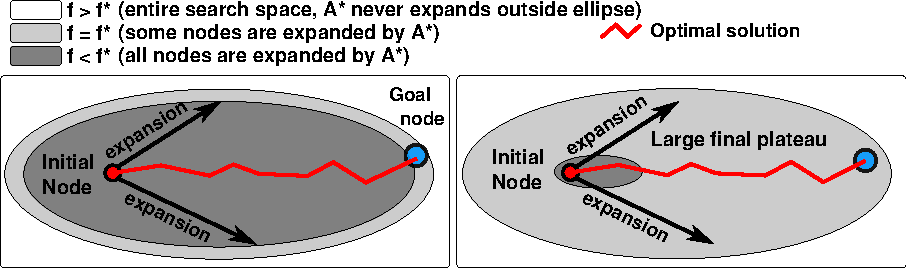
\includegraphics{img/astar/plateau-0.pdf}
% \caption{(Left) Naive understanding of the search space of \astar, which only holds for some limited domains. (Right) The reality of search spaces of combinatorial problems. The plateau containing the cost-optimal goals ($f=f^*$) is large, and it even accounts for most of the search effort required by \astar.
 \caption{(Left) One possible class of search space which is dominated by the states with cost $f<f^*$. (Right) This paper focuses on another class of search space, where the plateau containing the cost-optimal goals ($f=f^*$) is large, and it even accounts for most of the search effort required by \astar. % reworded to avoid offending all the SoCS people.
  }
 \label{fig:plateau-0}
\end{figure}

In the majority of such IPC problem domains where
the last layer ($f(n)=f^*$) accounts for a significant fraction of the effective search space, a
\emph{tiebreaking strategy}, which determines which node to expand among nodes with the same $f$-cost,
can have a significant impact on the performance of \astar.
It is widely believed that among nodes with the same $f$-cost,
ties should be broken according to $h(n)$, i.e.,
nodes with smaller $h$-values should be expanded first.  While this is a
useful rule of thumb in many domains, it turns out that tiebreaking
requires more careful consideration, particularly for problems where
most or all of the nodes in the last layer have the same $h$-value.

We empirically evaluate the existing, commonly used, standard
tiebreaking strategies for \astar (\refsec{sec:eval-common-strategies}).
We show that:

\begin{enumerate}
 \item A Last-In-First-Out (\lifo) criterion tends to be more efficient
       than a First-In-First-Out (\fifo) criterion.
 \item Tiebreaking according to the heuristic value $h$, which
       frequently appears in the heuristic search literature, has little
       impact on the performance as long as \lifo default criterion is used 
       --  in other words, a \lifo tiebreaking policy is sufficient for most IPC domains.
 \item There are significant performance differences among tiebreaking strategies
       when domains include zero-cost actions. This is true even when $h$-based tiebreaking is used.
\end{enumerate}

While there are currently relatively few standard benchmark domains with zero-cost actions,
we argue that zero-cost actions naturally occur in
practical cost-minimization problems.
Also, according to a parameterized complexity analysis, problem instances containing zero-cost actions are strictly harder than the instances with strictly positive action costs \cite{aghighi2015}.
Therefore, we introduce a new set of benchmarks called \emph{Zerocost domains}
(\refsec{sec:zerocost-domains}), which are a set of domains based on standard IPC domains for which only the most important actions which are directly related to resource usage incur non-zero cost.
We compare these domains with the original IPC domains from which they are derived, and empirically show that 
Zerocost domains have a different search space structure and different practical problem difficulty.

In order to solve such problems more efficiently, we propose and
evaluate \emph{depth diversification}, a new
tiebreaking method based on the notion of a node's \emph{depth} within a plateau,
which corresponds to the number of steps from the ``entrance'' to
the plateau (\refsec{sec:depth},
\refsec{sec:depth-based-evaluation}). 
Our new depth-based diversification strategy significantly improves upon the 
standard tiebreaking strategies.

We then propose a new framework which considers cost-optimal search using \astar 
as a series of satisficing searches on each plateau,
which allows the problem of tiebreaking to be reduced to satisficing search within a plateau (\refsec{sec:discussion}).
Based on this insight, we then investigate an
admissible tiebreaking strategy which uses the distance-to-go estimate, a heuristic function which treats every action
to have the unit costs (\refsec{sec:distance-to-go}).
Although distance-to-go estimates are inadmissible,
it does not harm the admissibility of entire search as long as it is used only for tiebreaking.
% 
We empirically show that:
\begin{enumerate}
 \item Tiebreaking using distance-to-go variations of \lmcut, \mands and \ff heuristics,
       with \lmcut or \mands as a primary heuristics for computing $f$ value (for maintaining admissibility),
       significantly improves the standard tiebreaking strategies.
       \todo*{listing 3 points regarding d2go might give the wrong impression that this paper is about d2go. combine some of the d2go bullets, or add another depth-related bullet?}
 % \item Distance-to-go variations of \emph{inadmissible} heuristics
 %       (\ff) further improves the performance by an order of magnitude.
 \item Combining depth-based diversification with distance-to-go heuristics 
       further improves the performance.
\end{enumerate}

% 

\begin{comment} % exclude if you want to submit a AAAI/ICAPS paper on satisficing 
In order to strengthen the connection between tiebreaking and satisficing search,
we also show a preliminary result that the depth diversification,
which was shown to improve tiebreaking performance,
also improves satisficing search using Greedy Best First Search (GBFS).
\end{comment}

\textbf{
Note for reviewers:
This paper is a significantly extended version of the AAAI-16 paper by
the same authors. The additions to the conference paper are the following:
\begin{enumerate}
 \item Introduction of deterministic depth-based diversification
       strategy (as opposed to the randomized version in the conference
       paper), and its theoretical analysis in \refsec{sec:depth}. 
 \item A new, thorough empirical analysis of the behavior of depth-based diversification in 
       \refsec{sec:depth-based-evaluation}.
 \item We propose a new framework for treating \astar as a sequence of satisficing searches on a set of $f$-cost plateaus (\refsec{sec:discussion}), and based on this new framework, we propose and evaluate tie-breaking strategies which incorporates distance-to-go estimates
       \refsec{sec:distance-to-go}.  
%Also, we included an empirical
%       evaluation of the use of inadmissible FF heuristics as part of
%       tiebreaking criterion, and its combination with the
%       depths metric thereof.
\end{enumerate}
Thus, over 50\% of \refsec{sec:depth}, as well as 100\% of \refsecs{sec:discussion}{sec:distance-to-go} are new.
% {[XXXTODO: Anything new (new experiments/data) in Sections 4??]}
}

